\documentclass[a4paper, 10pt]{article}
\usepackage[cm]{fullpage}


\usepackage{listings}
\usepackage{color}

\definecolor{mygreen}{rgb}{0,0.6,0}
\definecolor{mygray}{rgb}{0.5,0.5,0.5}
\definecolor{mymauve}{rgb}{0.58,0,0.82}

\lstset{ %
  backgroundcolor=\color{white},   % choose the background color; you must add \usepackage{color} or \usepackage{xcolor}
  basicstyle=\footnotesize,        % the size of the fonts that are used for the code
  breakatwhitespace=false,         % sets if automatic breaks should only happen at whitespace
  breaklines=true,                 % sets automatic line breaking
  captionpos=b,                    % sets the caption-position to bottom
  commentstyle=\color{mygreen},    % comment style
  deletekeywords={...},            % if you want to delete keywords from the given language
  escapeinside={\%*}{*)},          % if you want to add LaTeX within your code
  extendedchars=true,              % lets you use non-ASCII characters; for 8-bits encodings only, does not work with UTF-8
  frame=single,                    % adds a frame around the code
  keepspaces=true,                 % keeps spaces in text, useful for keeping indentation of code (possibly needs columns=flexible)
  keywordstyle=\color{blue},       % keyword style
  language=Octave,                 % the language of the code
  morekeywords={*,...},            % if you want to add more keywords to the set
  numbers=left,                    % where to put the line-numbers; possible values are (none, left, right)
  numbersep=5pt,                   % how far the line-numbers are from the code
  numberstyle=\tiny\color{mygray}, % the style that is used for the line-numbers
  rulecolor=\color{black},         % if not set, the frame-color may be changed on line-breaks within not-black text (e.g. comments (green here))
  showspaces=false,                % show spaces everywhere adding particular underscores; it overrides 'showstringspaces'
  showstringspaces=false,          % underline spaces within strings only
  showtabs=false,                  % show tabs within strings adding particular underscores
  stepnumber=2,                    % the step between two line-numbers. If it's 1, each line will be numbered
  stringstyle=\color{mymauve},     % string literal style
  tabsize=2,                       % sets default tabsize to 2 spaces
  title=\lstname                   % show the filename of files included with \lstinputlisting; also try caption instead of title
}
\usepackage{graphicx} % Required for the inclusion of images
\usepackage{natbib} % Required to change bibliography style to APA
\usepackage{amsmath} % Required for some math elements 

\setlength\parindent{0pt} % Removes all indentation from paragraphs

\title{Seismic Processing \\ Prac 3 - Review Questions} % Title

\author{ERTH3021} % Author name

\date{\today} % Date for the report

\begin{document}

\maketitle % Insert the title, author and date

\begin{figure}[h]
\centering
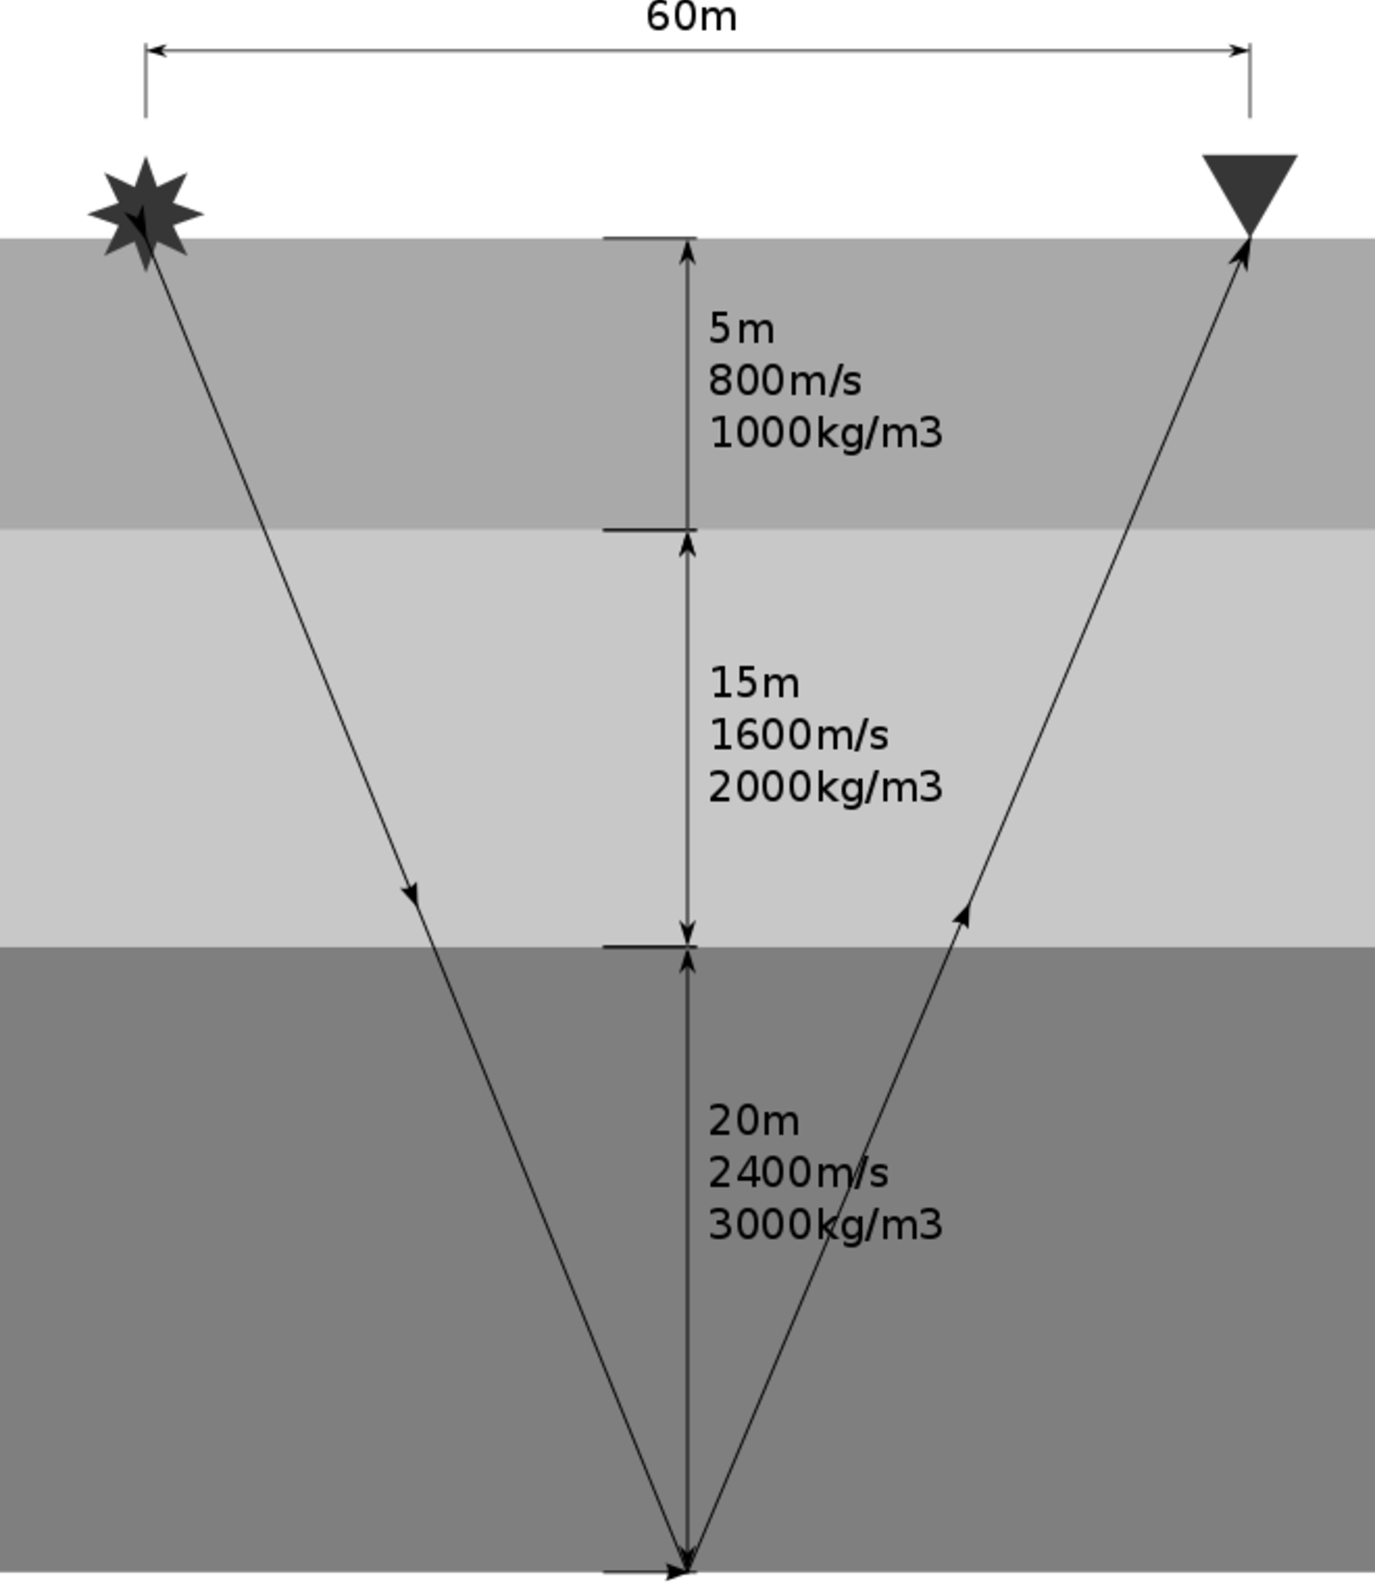
\includegraphics[width=0.8\textwidth]{model.pdf}
\caption{Seismic Model. The star is the source location and the triangle a geophone. This model assumes straight rays.}
\end{figure}
\newpage
\section{The Convolutional Model}
\subsection{}
Describe in words what convolution is, and how it differs from correlation. Give an example of where you might use a) convolution and b) correlation.
\subsection{}
The convolutional model of the seismic trace states that the trace we record is the result of the earth's response convolved with the source wavelet and the recording system, with some additional noise. Show an equation which describes this, and label each term.
\subsection{}
The earth's response consists of a range of different signals, including the direct wave, refracted wave and reflected wave.  Modify the convolutional model equation to include these signals.
\section{The Direct Wave}
\subsection{}
What is the direct wave?
\subsection{}
Assuming a velocity of 400m/s, how long does it take the direct wave to travel from the source to receiver shown in Figure 1?
\subsection{}
Attenuation of waves occurs for a number of reasons. One reason is that of spherical divergence. Describe the basic cause of amplitude loss due to spherical divergence.
\subsection{}
Briefly discuss one other cause of wave attenuation in seismic data.
\subsection{}
Assuming that the attenuation due to spherical divergence has a coefficient of two, and the source has unit amplitude, calculate the amplitude of the direct wave at the geophone in Figure 1.
\section{The Refracted Wave}
\subsection{}
What is a refracted wave? What is one potential use of the refracted wave data?
\subsection{}
What is the critical angle at the bottom of the first layer in the source-receiver geometry shown in Figure 1?
\subsection{}
What is the travel time for the geometry shown in Figure 1?
\newpage
\section{The Reflected Wave}
\subsection{}
Calculate the travel time of the reflected wave for the model shown in Figure 1. Assume straight rays.
\subsection{}
Discuss how you would analytically calculate the correct (non-straight) ray path.
\subsection{}
Assuming a unit source amplitude, calculate the amplitude of the reflected wave at the geophone due to transmission and reflection coefficients.  Assume zero offset coefficients.
\par~\\
Discuss when it might and might not be appropriate to use the zero offset assumption.

\section{Seismic Gathers}
\subsection{}
What is the difference between a shot gather, a receiver gather and  CMP gather? Draw a rough diagram of each.  
\subsection{}
What are CMP gathers useful for? Why?
\subsection{}
What assumptions are made when CMP stacking? What happens when these assumptions break down?
\subsection{}
What is fold?
\section{Amplitude Recovery}
\subsection{}
Why is amplitude recovery used?
\subsection{}
Why is using an AGC for amplitude recovery not ideal?
\section{Normal Moveout}
\subsection{}
Draw a rough diagram showing why normal moveout is hyperbolic.
\subsection{}
Calculate the zero offset travel-time for the reflection event in question 4.
\subsection{}
Wavelet stretching is caused by the non-linear NMO correction. Discuss the impact of stretch and a potential mitigation strategy.
\section{Stacking}
\subsection{}
What is stacking?  
\subsection{}
What is the signal to noise ratio improvement for a CMP gather with a fold of $n$?
\section{Noise attenuation}
\subsection{}
The refracted wave calculated in question 3 is often considered noise.  What is one method that can be used to remove the refracted wave? Discuss the steps required in this method.
\subsection{}
Often we want to enhance coherent events whilst attenuating random events. Discuss one method for achieving this. Discuss the potential negatives associated with this method.
\section{Processing Flows}
\subsection{}
Suggest a simple processing flow for a seismic dataset, using the processes discussed from question 5 to question 9.  State why you chose that particular processing sequence.  State any key parameters which need to be tested.

\newpage
\section{Useful Formulas}
\[R = \frac{1}{distance^2}\]
\[T = \frac{X}{V_1} + \frac{2z \cos{i_c}}{V_0}, \quad i_c = \sin^{-1}{\frac{V_0}{V_1}} \]
Where
\begin{itemize}
\item $X$ = lateral distance
\item $V_0$ = velocity of weathering layer
\item $V_1$ = velocity of sub-weathering layer
\item $z$ = thickness of weathering layer
\item $i_c$ = critical angle
\end{itemize}

\[ R_r = \frac{z_1 - z_0}{z_1+z_0}\]
\[ R_t = \frac{2*z_0}{z_1+z_0}\]
where 
\begin{itemize}
\item $z_0$  = acoustic contrast in layer 0, i.e. $\rho_0 v_0$
\item $z_1$ = acoustic contrast in layer 1, i.e. $\rho_1 v_1$
\end{itemize}

\[ {t_x}^2 = {t_0}^2 + \frac{x^2}{v^2}\]
where
\begin{itemize}
\item $t_x$ is the travel time at offset x
\item $t_0$ is the travel-time at offset 0
\item $x$ is the offset
\item $v$ is the velocity
\end{itemize}
\end{document}